% 固定的视觉回归样例，长题名和长院系名用于检查封面换行。
\documentclass{fduthesis}

\usepackage{amsmath}
\usepackage{booktabs}
\usepackage[backend=biber,style=gb7714-2025]{biblatex}
\addbibresource{reference.bib}

\fdusetup{
  type = academic,
  degree = master,
  title = {面向大规模有序数组的顺序查找与二分查找算法比较次数分析与评估},
  title-en = {Analysis and Evaluation of Comparison Counts for Linear and Binary Search Algorithms in Large Sorted Arrays},
  author = {张三}, student-id = {123456789},
  supervisor = {李四}, supervisor-title = {教授},
  committee = {李四教授, 王五副教授},
  major = {计算机科学与技术}, department = {空间信息科学与智能计算研究院城市环境感知与区域规划联合研究中心},
  date = {2026\hspace{0.5em}年\hspace{0.5em}6\hspace{0.5em}月\hspace{0.5em}30\hspace{0.5em}日},
  clc = {TP301.6},
  keywords = {有序数组, 二分查找, 算法分析},
  keywords-en = {sorted arrays, binary search, algorithm analysis},
  secret-level = {none},
}

\begin{document}
\frontmatter
\makecoverpage
\makecommittee
\tableofcontents

\begin{fdusummary}
在有序数组中查找一个键，顺序查找和二分查找各需访问多少个元素？
本文以七个互异整数为例，按目标键与数组元素的比较次数衡量查找代价。
当每个键被查询的概率相同时，顺序查找平均比较四次，二分查找平均比较 $17/7$ 次。
通过逐层统计二分查找判定树中的节点，还可得到任意非空数组的最坏比较次数。
\end{fdusummary}
\begin{fdusummaryen}
We count key comparisons in a sorted array of seven distinct integers.
When each key is equally likely to be queried, linear search uses four
comparisons on average, while binary search uses $17/7$.
The depth of the binary search decision tree also gives the worst-case
comparison count for an arbitrary nonempty array.
\end{fdusummaryen}
\listoffigures
\listoftables

\mainmatter
\chapter{有序数组的查找代价}
\section{比较次数的定义}
\makeatletter
\ifdim\f@size pt=12bp\else\errmessage{Expected 12bp body text}\fi
\makeatother
\ifdim\baselineskip=20bp\else\errmessage{Expected 20bp body leading}\fi
设数组按升序存储 $n$ 个互异的键。顺序查找从第一个元素向后扫描；
二分查找取当前区间的中点，根据比较结果保留左半区间或右半区间\cite{knuth1998}。
本文将目标键与一个数组元素的三路比较计为一次。%
\footnote{三路比较一次返回小于、等于或大于。若用两个条件判断实现，执行的判断指令数可能不同。}
一次未命中的中点比较至多留下 $\lfloor n/2\rfloor$ 个候选键。
因此，对非空数组，两种方法在成功查找时的最坏比较次数分别为
\begin{equation}
  C_{\mathrm{seq}}(n)=n,\qquad C_{\mathrm{bin}}(n)=\lfloor\log_2 n\rfloor+1 .
  \label{eq:worst}
\end{equation}

\subsection{按查询键计数}
对数组 $[1,2,3,4,5,6,7]$，表~\ref{tab:counts} 列出各键从开始查找到首次命中的比较次数。
两行的最大值分别为 7 和 3，与式~\eqref{eq:worst} 一致。
\begin{table}[htbp]
  \centering
  \caption{查找不同目标键所需的比较次数}
  \label{tab:counts}
  \begin{tabular}{lrrrrrrr}
    \toprule
    目标键 & 1 & 2 & 3 & 4 & 5 & 6 & 7 \\
    \midrule
    顺序查找 & 1 & 2 & 3 & 4 & 5 & 6 & 7 \\
    二分查找 & 3 & 2 & 3 & 1 & 3 & 2 & 3 \\
    \bottomrule
  \end{tabular}
\end{table}

\section{沿判定树查找}
图~\ref{fig:search} 中的每个节点都是一次中点选择。以查找键 5 为例：
\begin{enumerate}
  \item 先与根节点 4 比较，因 $5>4$，保留区间 $[5,7]$。
  \item 再与中点 6 比较，因 $5<6$，剩下的区间只含键 5。
  \item 与键 5 比较并命中，整个过程共比较三次。
\end{enumerate}
\begin{figure}[htbp]
  \centering
  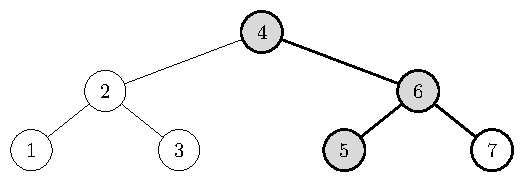
\includegraphics[width=.65\linewidth]{figures/figure1.pdf}
  \caption{二分查找判定树，灰色节点标出查找键 5 的路径}
  \label{fig:search}
\end{figure}
根节点 4 只需一次比较，而顺序查找对键 1 也只需一次比较。
要比较平均代价，还须给出各键被查询的概率，计算见附录~\ref{app:average}。

\printbibliography

\appendix
\chapter{等概率查询的平均代价}\label{app:average}
假设每次查询都成功，且七个键被查询的概率均为 $1/7$。
顺序查找的平均比较次数为 $(1+2+3+4+5+6+7)/7=4$。
在二分查找判定树中，第一、二、三层各有一、二、四个节点，
故平均比较次数为 $(1\times1+2\times2+4\times3)/7=17/7$。

\backmatter

\begin{acknowledgements}
感谢导师对查找算法示例和图表表达提出的建议。
\end{acknowledgements}
\makeauthorization
\end{document}
